%%%%%%%%%%%%%%%%%%%%%%%%%%%%%%%%%%%%%%%%%%%%%%%%%%%%%%%%%%%%%%%%%%%%%%%%%%%%%%
%
% PROJECT PROPOSAL  DESCRIPTION:
%   A concise description of the main concepts of the proposed project.
%
% RESEARCH:
%   A list of research activities which led to this project.
%
% EXPERIMENTS:
%   A list of the experiments performed which supported the research.
%
%%%%%%%%%%%%%%%%%%%%%%%%%%%%%%%%%%%%%%%%%%%%%%%%%%%%%%%%%%%%%%%%%%%%%%%%%%%%%%%
% Define a single space environment (copied from doublespace.sty)
% e.g. \begin{singlespace}
%         single-spaced text
%      \end{singlespace}

\documentclass[12pt,american]{article}

\usepackage{fullpage}
\usepackage{hyperref}
%\usepackage{bbm}
\usepackage{url}
%\usepackage{subfigure}
\usepackage{babel}
\usepackage{times}
\usepackage{graphicx}
\usepackage{amssymb}
%\usepackage{lscape}
\usepackage{verbatim}
\usepackage{enumerate}
%\usepackage{afterpage}
\usepackage{setspace}
%\usepackage{makeidx}
\usepackage{tabulary}
\usepackage{caption}
\usepackage{graphicx}
\usepackage{caption}
\usepackage{subcaption}
\usepackage{varwidth}
\usepackage{verbatim}
\usepackage{epigraph}

\newenvironment{centerverbatim}{%
  \par
  \centering
  \varwidth{\linewidth}%
  \verbatim
}{%
  \endverbatim
  \endvarwidth
  \par
}



\usepackage[round, sort&compress, authoryear]{natbib}

\newcommand{\quotes}[1]{``#1''}
\hypersetup{linktocpage}


\begin{document}
\thispagestyle{empty} 
\begin{center}
{\em MS Thesis Proposal}\\
\vspace{.5in}
{\large \bf Modeling of Distress: Towards Understanding Suicidaility}\\
\vspace{.5in}
{\bf Ravdeep Johar}\\
\vfill
\
{\em Committee Chair:} Dr. Cecilia Ovesdotter Alm\\
\vspace{0.1in}
{\em Reader: } Dr. Christopher M. Homan\\
 \vspace{0.1in}
{\em Observer: } Dr. Megan Lytle\\
 \vspace{0.1in}
Department of Computer Science\\
B. Thomas Golisano College of Computing and Information Sciences \\
Rochester Institute of Technology \\
Rochester, New York \\ [0.3in]
\vspace{0.5in}
\today{}\\
\end{center}
\vfill

%%%%%%%%%%%%%%%%%%%%%%%%%%%%%%%%%%%%%%%%%%%%%%%%%%%%%%%%%%%%%%%%%%%%%%%%%%%%%%%
%%  Collection of useful abbreviations.
\newcommand{\etc} {\emph{etc.\/}}
\newcommand{\etal}{\emph{et~al.\/}}
\newcommand{\eg}  {\emph{e.g.\/}}
\newcommand{\ie}  {\emph{i.e.\/}}
%%%%%%%%%%%%%%%%%%%%%%%%%%%%%%%%%%%%%%%%%%%%%%%%%%%%%%%%%%%%%%%%%%%%%%%%%%%%%%%


%%%%%%%%%%%%%%%%%%%%%%%%%%%%%%%%%%%%%%%%%%%%%%%%%%%%%%%%%%%%%%%%%%%%%%%%%%%%%%%
% Abstract
\section*{Abstract}
Suicide is a leading cause of death worldwide. One of the major challenges to suicide prevention is that those who may be most at risk cannot be relied upon to report their conditions to clinicians. This project will focus on modeling suicidaility using social media venues like Twitter, Reddit and TrevorProject. The modeling will provide an early flag system to identify users, who are at-risk using their social data.(wip) %The suicidality of a user is correlated with the distress (wip)
%%%%%%%%%%%%%%%%%%%%%%%%%%%%%%%%%%%%%%%%%%%%%%%%%%%%%%%%%%%%%%%%%%%%%%%%%%%%%%%
\vfill{}

%%%%%%%%%%%%%%%%%%%%%%%%%%%%%%%%%%%%%%%%%%%%%%%%%%%%%%%%%%%%%%%%%%%%%%%%%%%%%%%
% This is where the main body of the capstone proposal starts
\setcounter{page}{0} 
\newpage{}

\tableofcontents
\listoffigures
\listoftables

\pagebreak

\epigraph{When you get into a tight place and everything goes against you, till it seems as though you could not hang on a minute longer, never give up then, for that is just the place and time that the tide will turn.}{Harriet Beecher Stowe}

\section{Introduction}




Approximately a million people worldwide die by suicide every year \citep{who}, it is one of the leading causes of death among individuals aged 13-25 \citep{deaths}. Currently, there are no evidence based risk assessment tools for predicting or detecting suicidal behaviors and patients who seek help are assessed by the judgment of a psychological clinician, where the patient has to undergo a number of sessions to convey their distress. This leads to one of the major concerns while dealing with suicidality, that individuals, who are at risk, may not realize their level of risk or reach out for counseling, and even if they do,  will they be able to provide accurate information or express their distress?

Self-reporting cannot always be relied upon for detecting suicide ideation in patients. This thesis seeks to provide an additional way to assess the level of risk by utilizing a patient's social media information. Social media venues provide an informal setting, where people can interact and share their opinions without having any qualms about social stigma. In this informal setting, individuals may reveal their mental distress and even use such venues to seek support and guidance instead of clinical treatment \citep{bruffaerts2011treatment,ryan2010universal,crosby2011self}. 

Social media websites such as Twitter, Reddit and other micro-blogging services are attractive for research involving extracting and mining of text data. These websites produce a large volume of real-time data: Twitter has on average 140 million tweets posted everyday and Reddit generates about 40 million posts every year. The type of data varies with the website, from short updates (via tweets) to a long narration of personal experience (via Reddit). The quality of data is usually inconsistent, with informal register, non-standard text such as ad hoc abbreviations, phonetic substitutions, ungrammatical structures and usage of emoticons for expressiveness. These charatericts of social media data creates an additional challenge to semantically process the text data.

Prior research relevant to understanding suicidality has primarily been conducted in psychology to associate risk factors with suicidal behavior and is still under-studied. The stress-diathesis model by \cite{mann1999toward} provides evidence that risk factors such as depression, substance abuse or family violence can contribute to suicidal ideation. My research will focus on a preventive perspective of suicidaility rather than predicting if an individual will commit suicide. Specifically, this study aims to investigate if it is possible to automatically predict distress levels  (\textit{no distress, low distress} and\textit{ high distress}) based on users' social media information. Identifying users with such mental distress is an important step towards understanding and studying risk factors, which in the long term may help address suicide prevention by providing an early flagging system to identify individuals at-risk.



\section{Background}

Natural language processing(NLP) combines fields such as computer science, artificial intelligence and linguistics. It's concerned with understanding the human interactions using natural language. Although there huge advances in the field of Artificial Intelligence (AI) over the last few decades, the ultimate goal of making machines understand human language is still far off. 

\begin{comment}Historically, AI research concentrated on tasks that were considered intellectually hard and therefore impressive for humans: rapid calculations, verbatim memorization, playing chess at grandmaster level, automated theorem proving. Interestingly, these are all relatively simple to master for computers.
Early triumphs in these areas have inspired optimism that didn't translate to other fields, such as object recognition or understanding natural
language, which in turn led to repeated periods pessimism (known as the “AI winters”).


Talk about NLP \\
definitions of basic NLP terms \\
explain how using NLP to analyze text data is a CS task \\
Syntactic and Semantic processing \\
heirarchy and ambiguity \\
Applied science and social sciences \\
processing to understanding  \\
nlu is \\ 
more social data and
morphogical processing and named entities \\
semantic parsing \\
wsd wad \\
machine learning plays an important role and key techniques \\
importance of svm \\
\end{comment}

\section{Related Work}

Suicide is a subjective and complex phenomenon with a low base rate. Data on suicide is usually collected from healthcare organizations, large-scale studies, or self reporting \cite{crosby2011self,horowitz2009suicide}. The problem these sources is that they are limited by ociocultural barriers, such as stigma and shame \cite{crosby2011self}. Many researchers just focus on research related to associating risk factors and suicidaility without considering theoretical models \cite{nock2008suicide}. The know risk factors are Demographics, previous suicide attempts, mental health concerns (i.e., depression, substance abuse, suicidal ideation, self-harm, or impulsivity), family history of suicide, interpersonal conflicts (i.e., family violence or bullying), and mechanism, i.e., means for suicidal behavior (e.g., firearms). Any patient who exhibits more than three of these factors is considered to be at-risk.


\begin{comment}
Approximately one-third of all individuals who reported suicidal ideation in their lifetime made a plan to commit suicide. Nearly three-quarters of those who reported making a suicide plan actually attempted suicide \cite{kessler1999prevalence}. According to, the odds of attempting suicide increased exponentially when individuals endorsed three of more risk factors (e.g., having a mood or substance abused disorder). 
\end{comment}

The related work for this thesis can be categorized as research on: (nlp) suicide notes, social media and sentiment analysis.The earliest work on analyzing suicide notes was conducted by \cite{stone}, using a dataset of 750 real suicide notes collected over a period of 10 years,  they developed a system to detect real from simulated suicide notes(written by people from labor unions, fraternal groups, and the general community). Three patterns were observed:
\vspace{-0.2 mm}
\begin{itemize}
\itemsep-0.3em 
\item References to concrete things, persons and places were higher in real notes.
\item Usage of the word ``love'' was higher in real notes.
\item References to thought process and decision was higher in simulated notes.
\end{itemize} 
Recent work on suicide notes has involved classifying simulated and completer suicide notes \citep{pestinaetal2008,Pestian2}, the authors categorize the suicide notes into ideators(who think about suicide), attempters(who attempt suicde) and completers(who have completed suicide). They  utilize advanced techniques such as heterogeneous selection, parts-of-speech, Flesch and Kincaid readability score \citep{kincaid1975derivation} and various machine learning algorithms to show that these algorithms can perform on par with mental health professionals in this task of distinguishing simulated vs completer suicide notes.

Research on social media has recently gained a lot of attention due to the large amount of data it generates, the most interesting research capability of this data is forecasting: predicting future events. Researchers have successfully been able to predict election results \citep{gayo2013meta},  stock market movements \citep{bollen2011twitter}, flu outbreaks \citep{lampocris}, personality traits \citep{golbeck2011predicting},  mobility patterns of individuals \citep{song2010limits} and box-office revenues of movies \citep{asur2010predicting}. These predictive models although successful, are not perfect because text data can't entirely account for real-world outcomes. 

Sentiment Analysis is task of classifying the polarity of text into positive, neutral or negative. Early work consisted of  classifying movie reviews \citep{Pang} and product reviews \citep{Turney}  as positive or negative. \cite{Pang} and \cite{Snyder07multipleaspect} were then able to predict the ratings (based on 4, 5 or 10 point scale) of movies and restaurant based on their reviews. To classify these sentiments: Na\"ive Bayes, Maximum Entropy and SVM are the popular machine learning algorithms. Unlike traditional classifiers, where the neutral class is ignored, classifiers predicting sentiment are known to benefit with the addition of the neutral class. This task has of sentiment analysis can also classify human mood such as angry, happy or sad. \cite{read2005using} and \cite{Go} consider the usage of emoticons (such as :) and :-/) to predict sentiment of the text from Usenet newsgroups and Twitter using a dataset of positive and negative emoticons.

Software Libraries such as Linguistic inquiry and word count(LIWC)\citep{pennebaker2001linguistic} and SentiWordNet \citep{Baccianella} can classify a  given text data can various psycholinguistic categories such as work, anger, sad, happy, money, home, etc. LIWC provides 80 different categories, which can provide insight on an individuals social and psychological state-of-mind. 

Relatively less work has focused on suicide or other psychological conditions. \cite{ChoudhuryGCH13} and \cite{ponePrieto} successfully use Twitter data to detect depression and other mental health conditions, and argue that Twitter text data is viable to capture individuals psychological state. \cite{ChoudhuryGCH13} employed crowdsourcing to obtain a set of Twitter user who are clinically depressed based on standard psychometric tests. The author then retrieved  their social  information for last year and extracted behavioral text features and network features to predict the on-set of depression.

\cite{ponePrieto} attempts to predict health conditions such as flu, depression, pregnancy and eating disorders by extracting relevant tweets to each category using a set of regular expressions and then classifying these conditions using an SVM with mean f-measure of 0.85. 

\cite{Jay} used twitter data to identify suicide risk factors. The author used a filtering method to identify at-risk tweets using keywords and
phrases created from suicide risk factors. These at-risk tweets were then grouped by state and departures from expectation were calculated. This research provided evidence that suicide risk factors have a presence of twitter and research on suicide is viable using such data. 

\section{NLP Techniques}

\subsection{Text Normalization}

While dealing with text based data, it is first  preprocessed and/or normalized before any semantic processing can take place. 

\begin{itemize}
\item {Tokenization:} Splits text into individual words(tokens).
\item {Token Normalization:} Process of normalizing individual tokens by ignoring caps, removing punctuations or using a stemmer/lemmentizer. 
%\item {Spelling Correcter:}
\item {Replace Informal Register:} Using a dictionary of words collected from \url{noslang.com}, informal register is replaced with its meaning. For example, 'BBM' will be replaced with 'Black berry message'
\end{itemize}

\subsection{Bag of Words}

This is a common approach in NLP, where a sentence, for example: ``My name is Jon'' is represented as a set of words \{ 'My', 'name', 'is', 'Jon' \}.

\subsubsection{\emph{n}-gram Modeling}

Given a text, a \emph{n}-gram is  a contiguous sequence of \emph{n} items. It is called as uni-gram, bi-gram and tri-gram where $n=1,2,3$ respectively. For above example, the bi-gram model will be \{'My name', 'name is', 'is Jon'\}. Similary other \emph{n}-gram models can be created using the bag-of-words approach.




\subsection{Term Frequency-Inverse Document Frequency}

\emph{tf-idf} is a way to represent text data in a collection of documents using statistical weights. Each word in a document has a weight associated, which signifies the importance of the word in a document in the collection. The term frequency (tf) of a word (t) in a document (d) represented by equation ~\ref{eq:tf}, where $f(t,d)$ is the frequency of the term $t$ in document $d$. Since longer documents can cause a bias in the weighting, $tf$ is divided by the maximum frequency of a word in the document d.
\begin{equation}\label{eq:tf}
\mathrm{tf}(t,d) = 0.5 + \frac{0.5 \times \mathrm{f}(t, d)}{\max\{\mathrm{f}(w, d):w \in d\}}
\end{equation}
Inverse Document Frequency($idf$) is measure of how important a word is in the entire collection of documents and is calculated using equation ~\ref{eq:idf}, where, $N$ is the number of documents in the collection and $\frac{N}{|\{d \in D: t \in d\}|}$ is the number of documents in which the word($t$) occurs.
\begin{equation}\label{eq:idf}
 \mathrm{idf}(t, D) =  \log \frac{N}{|\{d \in D: t \in d\}|}
\end{equation}
\emph{tf-idf} is the multiplication of the above two terms(equation ~\ref{eq:tfidf}). This type of weighting is:
\begin{itemize}
\item Highest: when a word occurs many times within a small number of documents, which provides a discriminating power to these documents.
\item Lower: when the word occurs fewer times in a document, or occurs in many documents, which imples the word has no discrimination power or relevance.
\item Lowest: when the word occurs in all of the documents.
\end{itemize}
\begin{equation} \label{eq:tfidf}
 tf-idf = \mathrm{tf}(t,d)  * \mathrm{idf}(t, D)  
\end{equation}


\subsection{Latent Dirichlet Allocation}

Latent Dirichlet Allocation\citep{Blei} is an algorithm to perform Topic Modeling. It is an generative probabilistic model of a corpus of documents, where, the documents are  represented over a random mixture of latent topics and each topic is characterized over a distribution of words. 

\begin{figure}[h]
\fontsize{12}{4}\selectfont 
\begin{centerverbatim}
1. Choose N Poisson
2. Choose Dir.
3. For each of theN wordswn:
        (a) Choose a topic zn Multinomial().
        (b) Choose a wordwn from p(wn jzn;), 
            a multinomial probability conditioned on the topic
            zn.
\end{centerverbatim}
 \caption{Example input for annotator. }
\end{figure}


\begin{equation}
f \left(x_1,\cdots, x_{K-1}; \alpha_1,\cdots, \alpha_K \right) = \frac{1}{\mathrm{B}(\alpha)} \prod_{i=1}^K x_i^{\alpha_i - 1},
\end{equation}


\subsection{Support Vector Machine}

Support Vector Machine\citep{cortes} is a machine learning algorithm which can learn and recognize 	patterns. \citep{Aizerman67theoretical}


\begin{comment}
Formulate the problem as a math equation.
linear seperator \\
hyper plane \\
kernel trick important \\
non linear stuff \\

Topic models \\
understanding and semantics \\
reasoning and inferences \\

marriage between statistical and ai is strong with social media \\
text normalization (sproutz, goul et al )
(blei)
challenges is to interpereted results \\
supervised evaluation \\
challenges\\

express the hypothesis \\
\end{comment}

\section{Dataset}

I plan to make use of three datasets in the study. Two datasets have already been collected from Twitter. The first consists of  New York City tweets collected over a month, and the second consists of nationwide tweets. The third  dataset will be collected from Reddit using sub-reddits such as SuicideWatch, Depression, Happy, Anger, Selfharm, the goal is to collect about 2000 posts from each sub-reddit.  Another possible dataset consists of on-line chat support data from the Trevor Project, an organization that seeks to prevent suicide among LGBT teens. Access to the Trevor Chat dataset is in progress with support of a collaborator. 

\subsection{Human Subject Research}

RIT's IRB has confirmed that research involving Twitter or Reddit data, which is public, is not human subjects research, per federal definition. IRB approval for the Trevor Chat will be sought as soon as Trevor Project grants data access. My committee is experienced with human subjects research, and I have completed training in human subjects research.

\section{Current Work}

Currently, research already started on the first Twitter dataset, which consists of 2.5 million tweets. So far research has involved three steps: Filtering out distressed tweets, annotation and modeling. 


\subsection{Annotation}

The 2000 possible at-risk tweets were annotated by two novices and an expert, where the expert is a clinical psychologist with relevant experience in research with suicidality.The 2000 tweets were divided into two sets(1000 each). Novice one annotated the entire first set, novice two annotated 250 tweets from the first set and the expert annotated all the tweets in the second set. Each tweet was provided with a context of three tweets before and after the at-risk tweet, time stamps for all seven tweets and the thematic category to which the current tweet belongs to. Figure \ref{fig:example} provides an example of what each each tweet(as seen by the annotators). 
\begin{figure}[h]
\fontsize{9}{4}\selectfont 
\begin{centerverbatim}
978: Date: XXXX 
    -3: dat man on maury is overreacting!!
        he juss doin dat cuz he on 
        tv [-0:24:39]
    -2: @XXXX cedes!!! [-0:21:25]
    -1: yesssss! da weatherman was wronq 
        no rainy ass prom days!! yesss 
         prom is 2day guys!! class 
         of 2010! [-0:02:56]
>>> @XXXX awwww thanks trae-trae
     1: rt @XXXX: abt 2 hop in a kab 
        to skool i wouldn't dare spend 
        over 2 dollars to get somewhere
        i dnt wanna be n da first
        place! [+0:00:57]
     2: @XXXX yeaa [+0:03:59]
     3: @XXXX wassup? [+0:05:28]
Msg_id: XXXX  [Distress: ND, LIWC Sad: No]
\end{centerverbatim}
 \caption{Example input for annotator. The text within  "$>>>$" and "$<<<$"  is the current tweet}
 \label{fig:example}
\end{figure}
The annotators were asked to categorize the distress level on a four-point scale(as in table \ref{tab:distress}) and check if the tweet belonged to its thematic category or not. 
\begin{table}[h]
  \centering
  \begin{tabular}[h]{ll}
   \textbf{Code}&\textbf{Distress Level}\\
\hline
 H & happy \\
ND & no distress\\
 LD & low distress\\
HD &high distress
  \end{tabular}
  \caption{Distress-related categories used to annotate the tweets.}
  \label{tab:distress}
\end{table}
 Figure \ref{fig:distributions} shows the distributions of the annotations. An interesting observation is that, both novices were conservative/ reluctant to assign distressed labels compared to the expert. This shows that novices were unable pick up on subtly cues in the text that the expert could to identify tweets as distressed. Also the low number of happy tweets suggests that the filtering of tweets works well.



\begin{figure}
        \centering
        \begin{subfigure}[b]{0.4\textwidth}
               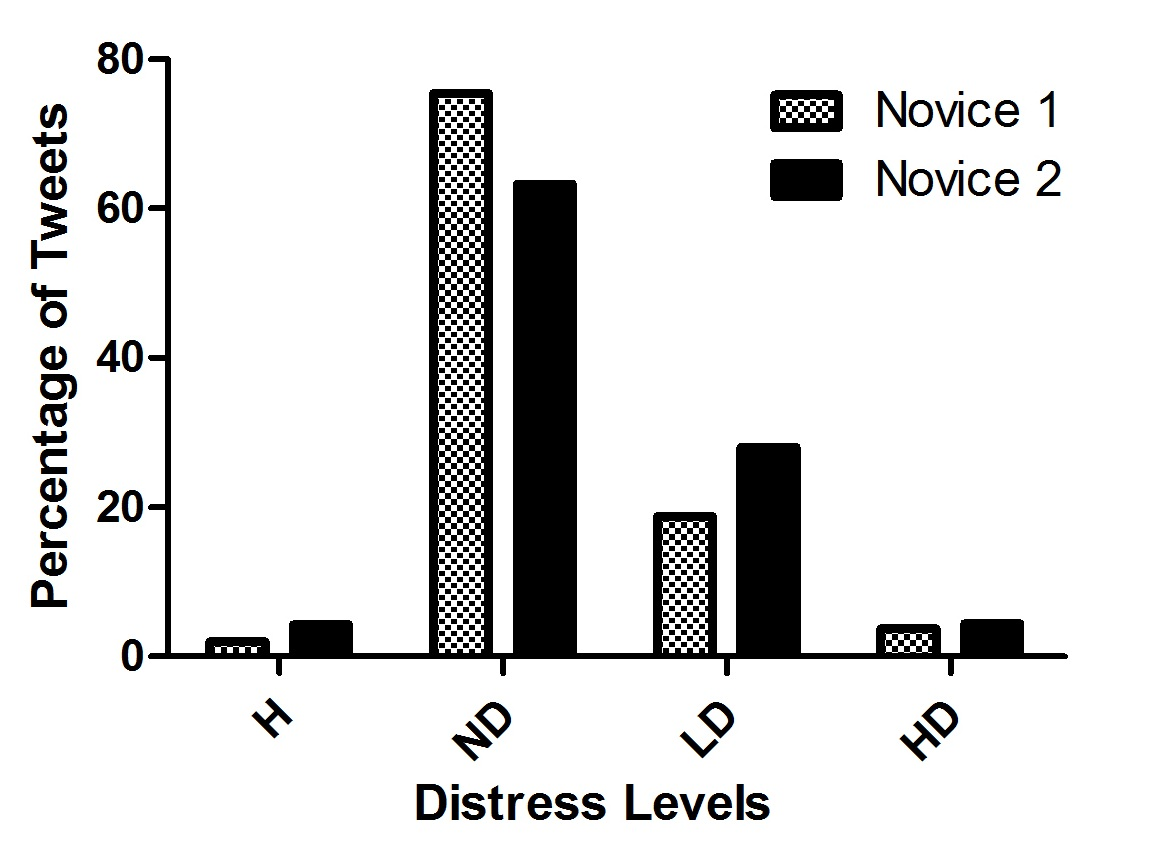
\includegraphics[width=\textwidth]{ChrisCissi4cat.jpg}
                \caption{Using tweets annotated by Novices 1 and 2 (N=250, identical set).}
                \label{fig:gull}
        \end{subfigure}%
        ~ %add desired spacing between images, e. g. ~, \quad, \qquad etc.
          %(or a blank line to force the subfigure onto a new line)
        \begin{subfigure}[b]{0.4\textwidth}
                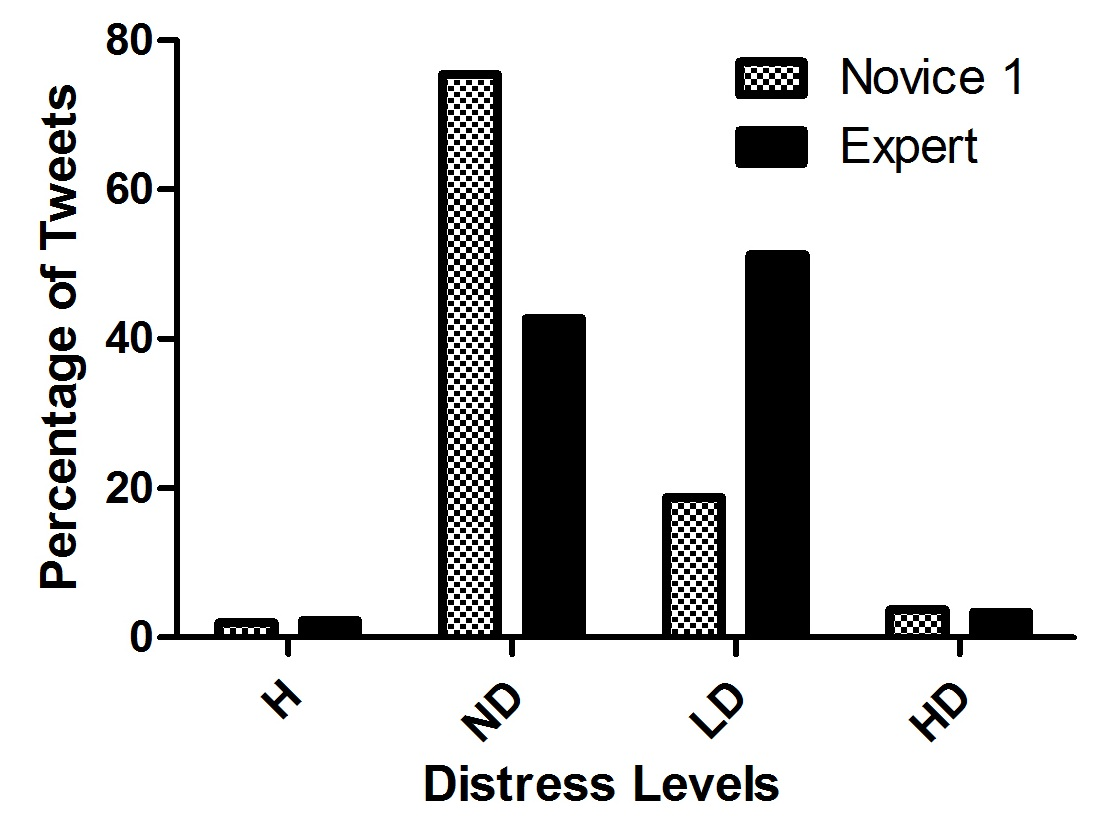
\includegraphics[width=\textwidth]{ChrisMegan4Cat.jpg}
                \caption{Using tweets annotated by Novice 1 and Expert. Note the these two datasets are disjoint (N = 1000 tweets, respectively)}
                \label{fig:tiger}
        \end{subfigure}     
\caption{Distribution of distress level annotations}
\label{fig:distributions}
\end{figure}




\subsection{Modeling and Results}

Topic Modeling:

\begin{table}[h]
\centering
\begin{tabular}{|>{\centering\arraybackslash}m{3in}| >{\centering\arraybackslash}m{3in}|}
\hline
High Distress & Random \\ \hline
feel like, wanna cry, get hurt, miss 2, ima miss, win lose, tired everything, broke bitches, gun range, one person & good morning, last night, happy birthday, look like, bout 2, can't wait, video , know (cont), chris brown, jus got \\ \hline
commit suicide, miss you!, miss baby, feel empty, committing suicide, tired living, sleep forever, lost phone, left alone, :( miss & feel like, let know, make sure, bout go, time get, don't get, wats good, . ., don't want, jus saw \\ \hline
hate job, feel sad, tummy hurts, lost friend, feel helpless, leave alone, don't wanna, worst feeling, leave world, don't let & don't know, let's go, looks like, what's good, go sleep, even tho, hell yea, new single, r u?, don't wanna \\ \hline
\end{tabular}
\caption{Topic analysis on bigrams of tweets labeled as high distress vs.\ randomly selected tweets from the larger, unlabeled dataset. The high distress tweets clearly convey strong negative affect.}
\label{tab:tm}
\end{table}

SVM:

\begin{table}[h]
\small \centering
\begin{tabular}{|c|c|c|c|c|}
\hline
Training         & Testing         & Precision & Recall & F-Measure \\ \hline
N1          & N1          & 0.53      & 0.63   & 0.58      \\ \hline
N1          & E & 0.58       & 0.27   & 0.37       \\ \hline
E           & E     & 0.59      & 0.71   & 0.64      \\ \hline
E            & N1          & 0.34      & 0.85   & 0.48      \\ \hline
N1 + E & N1 + E & 0.33      & 0.41   &  0.37         \\ \hline
\end{tabular}
\caption{Performance of SVM-based classification when the training and testing sets are alternately Novice 1 (N1) or the Expert (E). Because we focus on distress classification, we report precision, recall and F-measure for the distress class, which combines LD and HD into a single class with respect to  binary (distress vs.\ non-distress) classification. In each case, a held-out set of 100 randomly selected tweets compose the test set and the remaining 900 tweets from that annotator compose the training set. The last row shows when the two training sets (respectively, test sets) are combined into a single set of 1800 (respectively, 200) tweets. }
\label{tab:svm}
\end{table}



\section{Solution Design and Implementation}

\subsection{Visulizations}
\subsection{Social Network} 
\subsection{Modeling for Reddit Data} 
using topic modelling and other features 
\subsection{Outcome}
\section{Roadmap}

\subsection{Deliverables}

There will be two principal deliverables for this thesis. First, a thesis report and presentation describing the hypothesis, development, functionality, visualizations, results, evaluation and conclusion.  Second,  the code written for developing this system will be made available and reported for evaluation.    



\subsection {Timeline}


\begin{table}[h]
\centering
\begin{tabular}{l|l}
Date & Task \\ \hline
  15, 2014   & Complete thesis proposal   \\
 15, 2014   & Complete research work and implementation of algorithms  \\
 15, 2014   & Finish implementing the software \\
 15, 2014 & Finish writing report \\
 15, 2014 & Defense \\
\end{tabular}
\end{table}


\pagebreak

%%%%%%%%%%%%%%%%%%%%%%%%%%%%%%%%%%%%%%%%%%%%%%%%%%%%%%%%%%%%%%%%%%%%%%%%%%%%%%%

%%%%%%%%%%%%%%%%%%%%%%%%%%%%%%%%%%%%%%%%%%%%%%%%%%%%%%%%%%%%%%%%%%%%%%%%%%%%%%%
\bibliographystyle{apalike}
% Single space the bibliography to save space.
%\singlespacing
\bibliography{Proposal}
%%%%%%%%%%%%%%%%%%%%%%%%%%%%%%%%%%%%%%%%%%%%%%%%%%%%%%%%%%%%%%%%%%%%%%%%%%%%%%%


\end{document}
